\chapter{Lognormal Distribution ($X \sim \mathcal{LN}(\mu, \sigma^2)$) \cite{ism-1,wiki/Log-normal_distribution}} \label{Lognormal Distribution}

\begin{table}[H]
    \begin{minipage}{0.49\linewidth}
        \begin{figure}[H]
            \centering
            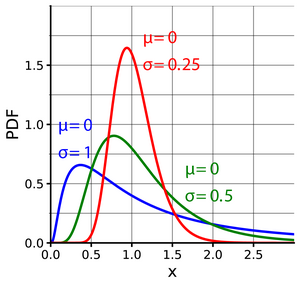
\includegraphics[width=\linewidth, height=4cm, keepaspectratio]{Pictures/distributions/Log-normal-pdfs.png}
            \caption{Lognormal distribution: PDF}
        \end{figure}
    \end{minipage}
    \hfill
    \begin{minipage}{0.49\linewidth}
        \begin{figure}[H]
            \centering
            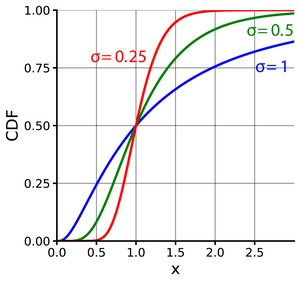
\includegraphics[width=\linewidth, height=4cm, keepaspectratio]{Pictures/distributions/Log-normal-cdfs.png}
            \caption{Lognormal distribution: CDF}
        \end{figure}
    \end{minipage}
\end{table}


\begin{alternateColorTable}
\renewcommand{\arraystretch}{2}
\begin{longtable}{|m{6cm}|p{9cm}|}
    \hline
    \tableHeaderRow
    \multicolumn{2}{|c|}{\textbf{Lognormal Distribution - Info} \cite{wiki/Log-normal_distribution}} \\
    \hline\endfirsthead

    \hline
    \tableHeaderRow
    \multicolumn{2}{|c|}{\textbf{Lognormal Distribution - Info - contd.} \cite{wiki/Log-normal_distribution}} \\
    \hline\endhead
    
    \hline\endfoot
    \hline\endlastfoot

    \hline
    \textbf{Notation} & 
    ${\displaystyle \ \operatorname {Lognormal} \left(\ \mu ,\,\sigma ^{2}\ \right)\ }$
    \\ \hline

    \textbf{Statistical parameters} & 
    \tableenumerate{
        \item ${\displaystyle \ \mu \in (\ -\infty ,+\infty \ )\ }$ (logarithm of location)

        \item ${\displaystyle \ \sigma >0\ }$ (logarithm of scale)
    }
    \\ \hline
    
    \textbf{Support} & 
    ${\displaystyle \ x\in (\ 0,+\infty \ )\ }$
    \\ \hline

    \textbf{Probability Density Function (PDF)} & 
    ${\displaystyle \ {\frac {1}{\ x\sigma {\sqrt {2\pi \ }}\ }}\ \exp \left(-{\frac {\left(\ln x-\mu \ \right)^{2}}{2\sigma ^{2}}}\right)}$
    \\[2ex] \hline
    
    \textbf{Cumulative distribution function (CDF)} & 
    ${\displaystyle \ {\frac {\ 1\ }{2}}\left[1+\operatorname {erf} \left({\frac {\ \ln x-\mu \ }{\sigma {\sqrt {2\ }}}}\right)\right]=\Phi \left({\frac {\ln(x)-\mu }{\sigma }}\right)}$
    \\ \hline

    \textbf{Quantile} &
    ${\displaystyle \ \exp \left(\mu +{\sqrt {2\sigma ^{2}}}\operatorname {erf} ^{-1}(2p-1)\right)\ }$
    \\ \hline

    \textbf{Mean} &
    ${\displaystyle \ \exp \left(\ \mu +{\frac {\sigma ^{2}}{2}}\ \right)\ }$
    \\ \hline

    \textbf{Median} & 
    ${\displaystyle \ \exp(\ \mu \ )\ }$
    \\ \hline

    \textbf{Mode} & 
    ${\displaystyle \ \exp \left(\ \mu -\sigma ^{2}\ \right)\ }$
    \\ \hline

    \textbf{Variance} &
    ${\displaystyle \ \left[\ \exp(\sigma ^{2})-1\ \right]\ \exp \left(2\ \mu +\sigma ^{2}\right)\ }$
    \\ \hline

    \textbf{Skewness} &
    ${\displaystyle \ \left[\ \exp \left(\sigma ^{2}\right)+2\ \right]{\sqrt {\exp(\sigma ^{2})-1\;}}}$
    \\ \hline

    \textbf{Excess kurtosis} &
    ${\displaystyle \ 1\ \exp \left(4\ \sigma ^{2}\right)+2\ \exp \left(3\ \sigma ^{2}\right)+3\ \exp \left(2\sigma ^{2}\right)-6\ }$
    \\ \hline

    \textbf{Entropy} &
    ${\displaystyle \ \log _{2}\left(\ {\sqrt {2\pi \ }}\ \sigma \ e^{\mu +{\tfrac {1}{2}}}\ \right)\ }$
    \\[1ex] \hline

    \textbf{Characteristic function (CF)} &
    representation ${\displaystyle \ \sum _{n=0}^{\infty }{\frac {\ (i\ t)^{n}\ }{n!}}e^{\ n\mu +n^{2}\sigma ^{2}/2}\ }$ is asymptotically divergent, but adequate for most numerical purposes
    \\[1ex] \hline

    \textbf{Method of moments} &
    \tableenumerate{
        \item ${\displaystyle \ \mu =\log \left({\frac {\operatorname {\mathbb {E} } [X]\ }{\ {\sqrt {{\dfrac {\ \operatorname {Var} [X]~~}{\ \operatorname {\mathbb {E} } [X]^{2}\ }}+1\ }}\ }}\right)\ }$
        \vspace{0.1cm}

        \item ${\displaystyle \ \sigma ={\sqrt {\log \left({\dfrac {\ \operatorname {Var} [X]~~}{\ \operatorname {\mathbb {E} } [X]^{2}\ }}+1\ \right)\ }}}$
        \vspace{0.1cm}
    }
    \\[1ex] \hline

    \textbf{Expected shortfall} &
    ${\displaystyle \ {\dfrac {\ \operatorname {erfc} \left({\dfrac {s}{\ {\sqrt {2\ }}\ }}-\operatorname {erf} ^{-1}(2p-1)\right)\ }{2}}(1-p)e^{\mu +{{~s^{2}\ }/{2}}}\ }$
    \\[2ex] \hline

    \textbf{relative standard deviation} & 
    $\sqrt{e^{\sigma^2} - 1}$
    \\[1ex] \hline

\end{longtable}
\renewcommand{\arraystretch}{1}
\end{alternateColorTable}


\begin{enumerate}[itemsep=0.2cm]
    \item the lognormal PDF is \textbf{NOT SYMMETRIC} like the normal PDF 

    \item If the population values can be described by a lognormal PDF, the normal PDF would then describe the logarithmic transformation of the population values (using the natural logarithm)

    \item Parameters:
    \begin{table}[H]
        \centering
        \begin{tabular}{l l l}
            $\mu$ & population mean   & $(\mu \in R)$ \\
            
            $\sigma$ & standard deviation &   $(\sigma^2 > 0)$ \\
            
            $x > 0$ & & \\

        \end{tabular}
    \end{table}

    \item They do represent the population mean and standard deviation, but only for the logarithmic transformed values of the population

    \item if $X_1, X_2,\cdots, X_n$ are i.i.d. lognormally distributed, then transformed random variables $\log(X_1), \log(X_2),\cdots, \log(X_n)$:
    \begin{enumerate}[itemsep=0.2cm]
        \item (transformed) sample average:
        \[
            \bar{X}_{\log} = \dfrac{1}{n} \dsum_{i=1}^n \log(X_i)
            \hfill
            \bar{X}_{\log} \sim \mathcal{N}(\mu, \sigma^2/n)
        \]

        \item (transformed) sample variance:
        \[
            S_{\log}^2 = \dfrac{1}{n-1} \dsum_{i=1}^n (\log(X_i) - \bar{X}_{\log})^2
            \hspace{3cm}
            (n-1)S_{\log}^2/\sigma^2 \sim \chi_{n-1}^2
            \ (DOF=n-1)
        \]

        \item These sample statistics are unbiased estimates of $\mu$ and $\sigma^2$

        \item (transformed) geometric average:
        \[
            \exp(\bar{X}_{\log}) = \dprod_{i=1}^n \sqrt[n]{X_i}
        \]

    \end{enumerate}

\end{enumerate}


\section{Probability Density Function (PDF) ($f_{\mu,\sigma}(x)$) \cite{ism-1}} \label{Lognormal Distribution: PDF}

\[
    f_{\mu,\sigma}(x)
    = \begin{cases}
        \dfrac{1}{x\sigma\sqrt{2\pi}}
        \exp\dCurlyBrac{-\dfrac{(\log(x) - \mu)^2}{2\sigma^2}} & x > 0 \\[2ex]
        
        0 & x \leq 0
    \end{cases}
\]


\section{Cumulative Distribution Function (CDF) \cite{ism-1}} \label{Lognormal Distribution: CDF}

\begin{align*}
    Pr(\exp\dCurlyBrac{X} \leq x) 
    &= Pr(X \leq \log(x))
    = \phi\dParenBrac{\dfrac{\log(x) - \mu}{\sigma}} \\
    &= \dint_{-\infty}^{\log(x)} \dfrac{1}{\sigma}
        \phi\dParenBrac{\dfrac{z - \mu}{\sigma}} dz
    = \dint_{-\infty}^{x} \dfrac{1}{z\sigma}
        \phi\dParenBrac{\dfrac{\log(z) - \mu}{\sigma}} dz \\
\end{align*}


\section{Method of Moments Estimation (MME) \cite{ism-1}} \label{Lognormal Distribution: MME}
\begin{enumerate}[itemsep=0.2cm]
    \item population density: $
        f_L(x) 
        = \dfrac{1}{[x\sigma]} \phi\dParenBrac{
            \dfrac{[\log(x) - \mu]}{\sigma}
        }
    $ \hfill ($x > 0$)

    \item parameters: 
        $\theta_1 = \mu$ 
        and 
        $\theta_2 = \sigma^2$
    
    \item Equations:
    \begin{enumerate}[itemsep=0.2cm]
        \item $
            \bar{X}
            = \mu(f_L)
            = \exp(\mu + 0.5\sigma^2)
        $

        \item $
            M_2
            = \sigma^2(f_L)
            = \exp(2\mu + \sigma^2)(\exp(\sigma^2) - 1)
        $

        \item $
            \dfrac{\sigma^2(f_L)}{\mu^2(f_L)}
            = \exp(\sigma^2) - 1
        $

    \end{enumerate}

    \item solutions:
    \begin{enumerate}[itemsep=0.2cm]
        \item $
            \tilde{\sigma}^2
            = \log\dParenBrac{1 + \dfrac{M_2}{\bar{X}^2}}
            = \log\dParenBrac{\bar{X}^2 + {M_2}} - 2\log\dParenBrac{\bar{X}}
        $

        \item $
            \tilde{\mu}
            = \log\dParenBrac{\bar{X}} - 0.5[\log\dParenBrac{\bar{X}^2 + {M_2}} - 2\log\dParenBrac{\bar{X}}]
            = 2\log\dParenBrac{\bar{X}} - 0.5\log\dParenBrac{\bar{X}^2 + {M_2}}
        $

    \end{enumerate}

    \item Alternative approach:
    \begin{enumerate}[itemsep=0.2cm]
        \item considered the set of transformed random variables $\log(X_1), \log(X_2),\cdots, \log(X_n)$

        \item These random variables are normally distributed with mean $\mu$ and variance $\sigma^2$

        \item $
            \hfill 
            \tilde{\mu} = \bar{X}_{\log}
            \hfill
            \tilde{\sigma}^2 = (n-1)S_{\log}^2/n
            \hfill
        $

    \end{enumerate}

\end{enumerate}



\section{Maximum Likelihood Estimation (MLE) \cite{ism-1}} \label{Lognormal Distribution: MLE}
\begin{enumerate}[itemsep=0.2cm]
    \item population density: $
        f_L(x) 
        = \dfrac{1}{[x\sigma]} \phi\dParenBrac{
            \dfrac{[\log(x) - \mu]}{\sigma}
        }
    $ \hfill ($x > 0$)

    \item parameters: 
        $\theta_1 = \mu$ 
        and 
        $\theta_2 = \sigma^2$

    \item standard normal density: $
        \phi(x) = \dfrac{1}{\sqrt{2\pi}} \exp\dParenBrac{-\dfrac{x^2}{2}}
    $

    \item log likelihood: $
        \dsum_{i=1}^{n} \log(f_L(X_i))
        = \dsum_{i=1}^{n} \dSquareBrac{
            -\dfrac{(\log(X_i) - \mu)^2}{2\sigma^2}
            -\log(\sqrt{2\pi})
            -\log(X_i)
            -\log(\sigma)
        }
    $
    
    \item likelihood equations: 
    \begin{enumerate}[itemsep=0.2cm]
        \item $
            \dsum_{i=1}^{n} \dSquareBrac{\dfrac{\log(X_i) - \mu}{\sigma^2}} = 0
        $

        \item $
            \dsum_{i=1}^{n} \dSquareBrac{
                \dfrac{(\log(X_i) - \mu)^2}{\sigma^3}
                - \dfrac{1}{\sigma}
            } = 0
        $

    \end{enumerate}

    \item solutions:
    \begin{enumerate}[itemsep=0.2cm]
        \item $
            \hat{\mu}
            = \bar{X}_{\log}
            = \dsum_{i=1}^n \log(X_i)
        $

        \item $
            \hat{\sigma}^2
            = \dfrac{1}{n} \dsum_{i=1}^{2} (\log(X_i) - \bar{X}_{\log})^2 
            = (n-1)S_{\log}^2/n
        $

        \item $
            \mathbb{E}(\hat{\sigma}^2)
            = \mathbb{E}((n-1)S_{\log}^2/n) 
            = (n-1)\sigma^2/n
        $ \\
        (bias vanishes when the sample size gets large)

    \end{enumerate}

    \item MLE estimate: $
        \exp(\hat{\mu} + 0.5\hat{\sigma}^2) 
    $

\end{enumerate}


\section{Bivariate \cite{ism-1}} \label{Lognormal Distribution: Bivariate}

\begin{enumerate}
    \item Assumption:
    \begin{enumerate}
        \item $X \sim \mathcal{N}(\mu_X, \sigma_X^2)$

        \item $Y \sim \mathcal{N}(\mu_Y, \sigma_Y^2)$

        \item $\rho$: dependency parameter

        \item $X + Y$ has a normal distribution
        \begin{enumerate}
            \item mean: $\mu_X + \mu_Y$

            \item variance: $\sigma_X^2 + 2\rho\sigma_X\sigma_Y + \sigma_Y^2$
        \end{enumerate}

    \end{enumerate}

    \item $(exp(X), exp(Y))$ has a bivariate lognormal distribution

    \item covariance:
    \begin{enumerate}
        \item 
        \begin{align*}
            COV(exp(X), exp(Y )) 
            &= E[exp(X) exp(Y )] - E[exp(X)]E[exp(Y )] \\
            &= E[exp(X + Y )] - exp(\mu_X + 0.5\sigma^2_X ) exp(\mu_Y + 0.5\sigma^2_Y ) \\
            &= exp(\mu_X + \mu_Y + 0.5(\sigma^2_X + 2\rho\sigma_X \sigma_Y + \sigma^2_Y ))
                 -exp(\mu_X + 0.5\sigma^2_X ) exp(\mu_Y + 0.5\sigma^2_Y ) \\
            &=exp(\mu_X + 0.5\sigma^2_X + \mu_Y + 0.5\sigma^2_Y )(exp(\rho\sigma_X \sigma_Y ) - 1) \\
            &= E[exp(X)]E[exp(Y )](exp(\rho\sigma_X \sigma_Y ) - 1)
        \end{align*}

        \item $COV(X, Y) = \rho\sigma_X\sigma_Y$
    \end{enumerate}

    
\end{enumerate}

\section{Pearson’s correlation coefficient ($\rho_P$) \cite{ism-1}} \label{Lognormal Distribution: Pearson’s correlation coefficient}

\begin{enumerate}[itemsep=0.2cm]
    \item variances:
    \begin{enumerate}[itemsep=0.2cm]
        \item exp(X) : $(E[exp(X)])2(exp(\sigma_X^2) - 1)$

        \item exp(Y) : $(E[exp(Y)])2(exp(\sigma_Y^2) - 1)$

    \end{enumerate}

    \item covariance: $E[exp(X)]E[exp(Y)](exp(\rho\sigma_X\sigma_Y) - 1)$

    \item Pearson’s correlation coefficient: $
        \rho_P
        = \dfrac{exp(\rho\sigma_X \sigma_Y ) - 1}{\sqrt{(exp(\sigma^2_X ) - 1)(exp(\sigma^2_Y ) - 1)}}
    $

    \item When the variances of $X$ and $Y$ are the same, say $\sigma _X^2 = \sigma _Y^2 = \sigma ^2$
    \begin{enumerate}
        \item $\rho _P = \dfrac{exp(\rho \sigma 2) - 1}{exp(\sigma 2) - 1}$

        \item correlation is relatively constant for the variance $\sigma ^2 \leq 1$

    \end{enumerate}
\end{enumerate}





































